\documentclass[../dissertation.tex]{subfiles}
\begin{document}

\chapter{Testing and Evaluation}

\section{Testing}

\subsection{Unit Testing}

Unit testing was conducted on the two main components of the Tulip Web Wrapper, along with on the views responsible for returning the HTML to the client. 

\subsubsection{Conversion from \texttt{.tlp} to \texttt{.json}}

To confirm that the conversion from a Tulip graph to a JSON object was successful, tests were created for several different networks. The set up of the tests included loading three network from a file into memory using Tulip's \texttt{tlp.loadGraph()}. Then, on each of the networks, the conversion code was run and it was checked that the number of nodes and edges was correct, with the function \texttt{TlpJsonConverter.tlp\_to\_json()}.

\subsubsection{Confirming all of the bundling algorithms work}

To test each algorithm initially three different networks were loaded into the system using Tulip's \texttt{tlp.loadGraph()}. One of these networks would be used to test Node Bundling based on cliques (as it was a very interconnected network) and the other two networks would be used to test Node Pruning and Node Bundling based on number of edges, being far more sparsely connected networks. Each test consisted of checking the number of nodes upon loading in the network, applying the appropriate operation that was being tested for, and then confirming that the number of nodes and edges returned from the function was as expected.

\subsubsection{Successful page responses}

The unit tests that confirmed that both the part of the back-end that returned data to the front-end worked by creating a fake call to the server using a GET or POST request as appropriate and that the Tulip Web Wrapper worked as appropriate. This was done by checking that the calls were successful and either returned a status code of 200 if a \texttt{HttpResponse} was returned, or included success = True if a \texttt{JsonResponse} was returned.

\subsection{Integration Testing}

The integration tests for the Tulip Web Wrapper involved creating a network in the database during the set up phase of the test and then loading in that network using different algorithms and ensuring the output at the end was correct. This entailed calling the \texttt{loadGraph} API call and passing in appropriate parameters such as the network name, and whether node pruning or node bundling using number of edges was enabled. The response of that call (a JSON object) was then decoded and it was checked if the call had been successful, and if it had contained the correct number of nodes and edges, along with the expected number of nodes that had been pruned of bundled. This ensured that the logic within the view was correct, that the bundling code worked as expected, and that the conversion worked as expected.

\section{User Evaluation}

Not appropriate as the main goal was to optimise performance and a very basic interface was created. However, on further development of this project, a full user evaluation would be conducted.

\section{Performance Evaluation}

\subsection{Aim}

The goal of the performance evaluation was to thoroughly test the system that had been created. This would involve loading several different networks into the system, and then recording the performance of the system when different algorithms are used and comparing the results.

\subsection{Methodology}

As SAS had provided four different networks to utilise, they would be used to conduct the evaluation on. The networks had approximately thirty, two hundred, one thousand and three thousand nodes respectively, and always a similar number of edges. Each of these networks would first be uploaded into the system and then rendered with the following parameters: no algorithm set, node pruning, node bundling based on number of edges and both node pruning then node bundling based on number of edges.

The runs were conducted on the same machine, one by one, while no other application was running apart from the Django development server which hosted the site. Each run of the evaluation was done five times so a reliable average could be taken. For each run, the following information was collected:

\begin{itemize}
    \item Client-Side:
    \begin{itemize}
        \item The time taken between the user clicking `Load' and the client getting an AJAX response back - This was recorded to discover how long the JavaScript took to respond, call the server using AJAX, and get a response - essentially recording the time spend processing the network and sending it across the network.
        \item The time spent processing the data got from the AJAX call and formatting it for Vis.js - The reason this was recorded was to find out how long it took for JavaScript to process the data and format it appropriately for Vis.js, which included adding all of the nodes and edges to a list and then setting properties (such as size, shape and colour) appropriately.
        \item The time spent creating Vis.js network - How long it took to create the network in memory from the list of nodes and edges, and any \texttt{options} parameters set such as physics models.
        \item The time spent rendering the network - Depending on what \texttt{options} are set for Vis.js, this can be as simple as loading each node in a ring, equally spaced apart, and drawing in the edges appropriately. However, it is far more useful to have a force directed network in which each node exerts a force and several constants are set, and the model is left to settle before it is shown to the user. The latter is what was chosen for the performance evaluation.
    \end{itemize}
    \item Server-Side:
    \begin{itemize}
        \item The time taken to load in the requested \texttt{.tlp} file from the database into Tulip - This represents how long it takes for the network to be located in the database, loaded in to memory and then loaded in to Tulip as a Graph object.
        \item (if applicable) How long pruning the network took - The length of time taken to loop over the network and prune it as appropriate, and return both the modified network and a list containing each node that has been pruned and how many nodes have been removed from it.
        \item (if applicable) How long node bundling based on the number of edges took - The time taken to decide what nodes should be bundled and to then bundle them, while tracking how many nodes have been removed from each bundled node.
    \end{itemize}
    \item Network Information:
    \begin{itemize}
        \item The number of nodes in the network.
        \item The number of edges in the network.
        \item How many bytes the packet contains that is to be sent across the network.
    \end{itemize}
    \item Total Time:
    \begin{itemize}
        \item The total time taken from the user clicking `Load' to the network rendering.
        \item The standard deviation of the total time.
    \end{itemize}
\end{itemize}

\subsection{Results and Discussion}

The following four tables show the effect of different algorithms on different networks. Each table shows the total time taken to load, manipulate and render the network, and how much data was sent. Table \ref{table:30-nodes} shows the results for a network with thirty nodes, Table \ref{table:200-nodes} shows the results for two hundred nodes, Table \ref{table:1000-nodes} shows the results for one thousand nodes and Table \ref{table:3000-nodes} shows the results for three thousand nodes.

\subsubsection{30 Nodes}

Node Pruning resulted in a 50\% decrease in total time to visualise, and 36\% decrease in packet size, compared to applying no algorithm.
Node Bundling based on the number of edges resulted in a 24\% decrease in time generate and render, and 36\% decrease in packet size, compared to not applying an algorithm. Applying both Node Pruning and Node Bundling based on number of edges resulted in a 63\% decrease in amount of time to visualise and a 40\% decrease in packet size. Node Pruning is clearly more effective than Node Bundling, providing lower packet sizes and faster network loading times.

\begin{table}[H]
\centering
\begin{tabular}{|l|l|l|l|l|}
\hline
                    & \textbf{None}    & \textbf{Pruning} & \textbf{Edge-based Bundling}    & \textbf{Both}   \\ \hline
Total Time (ms)     & 170.8 $\pm$ 15.3 & 85.8 $\pm$ 20.5  & 129.6 $\pm$ 19.3 & 63.2 $\pm$ 15.2 \\ \hline
Packet Size (bytes) & 1300             & 827              & 1012             & 785             \\ \hline
\end{tabular}
\caption{Total Times to load a network of 30 nodes and size of packet transferred over the network}
\label{table:30-nodes}
\end{table}

\subsubsection{200 Nodes}

For 200 nodes, Node Pruning provides a 91\% decrease in total load time and a 49\% decrease in packet size compared to no algorithm being applied. For Node Bundling based on number of edges, the decrease in load time was 9\% and the packet size decreased by 20\%. Applying Node Pruning followed by Node Bundling based on number of nodes resulted in a 98\% decrease in loading times and a 70\% decrease in packet size. Node Pruning is again more effective at lowering the amount of data that needs to be transferred and lowering the amount of time to manipulate and render the network.

\begin{table}[H]
\centering
\begin{tabular}{|l|l|l|l|l|}
\hline
                    & \textbf{None}       & \textbf{Pruning}  & \textbf{Edge-based Bundling}       & \textbf{Both}    \\ \hline
Total Time (ms)     & 7382.8 $\pm$ 2010.2 & 663.0 $\pm$ 187.0 & 6749.0 $\pm$ 1075.0 & 146.6 $\pm$ 14.5 \\ \hline
Packet Size (bytes) & 7600                & 3900              & 6100                & 2300             \\ \hline
\end{tabular}
\caption{Total Times to load a network of 200 nodes and size of packet transferred over the network}
\label{table:200-nodes}
\end{table}

\subsubsection{1000 Nodes}

When the network with 1000 nodes was used, similar results to above were seen. There was an 84\% decrease in loading times and 51\% decrease in packet size for Node Pruning, and a 36\% decrease in loading times and a 29\% decrease in packet size in comparison to not applying any algorithm to the network. When applying both Node Pruning then Node Bundling based on the number of edges, the decrease in loading times was 99.997\% and the packet size was reduced by 70\%. Again, Node Pruning was shown to be more effective than Node Bundling based on number of edges, but additionally there was a massive decrease in loading times when applying both algorithms.

\begin{table}[H]
\centering
\begin{tabular}{|l|l|l|l|l|}
\hline
                    & \textbf{None}        & \textbf{Pruning}    & \textbf{Edge-based Bundling}        & \textbf{Both}    \\ \hline
Total Time (ms)     & 59924.4 $\pm$ 8343.5 & 9417.8 $\pm$ 2223.1 & 38139.8 $\pm$ 9383.0 & 152.6 $\pm$ 30.5 \\ \hline
Packet Size (bytes) & 41400                & 20300               & 29400                & 12400            \\ \hline
\end{tabular}
\caption{Total Times to load a network of 1000 nodes and size of packet transferred over the network}
\label{table:1000-nodes}
\end{table}

\subsubsection{3000 Nodes}

For the largest network, with 3000 nodes, results were as follow. Loading times decreased by 81\% and packet size decreased by 44\% for Node Pruning when compared to using no algorithm. For Node Bundling based on number of edges, a decrease of 48\% was seen for loading times and a 27\% decrease was seen for packet size next to using no algorithm. When applying Node Pruning followed by Node Bundling based on number of edges the decrease in total time was 94\%, and the decrease of packet size was 72\%. Similar to above, a performance increase was most notable for Node Pruning. 

\begin{table}[H]
\centering
\begin{tabular}{|l|l|l|l|l|}
\hline
                    & \textbf{None}          & \textbf{Pruning}     & \textbf{Edge-based Bundling}         & \textbf{Both}        \\ \hline
Total Time (ms)     & 252849.2 $\pm$ 32862.0 & 48956.8 $\pm$ 3937.0 & 131606.6 $\pm$ 6031.3 & 14532.8 $\pm$ 3341.0 \\ \hline
Packet Size (bytes) & 114000                 & 63500                & 83500                 & 42900                \\ \hline
\end{tabular}
\caption{Total Times to load a network of 3000 nodes and size of packet transferred over the network}
\label{table:3000-nodes}
\end{table}

Figure \ref{fig:loadTimes} shows the total load times for each of the different networks and each of the different algorithms. It can clearly be seen that Node Bundling based on number of edges is less effective than Node Pruning for all network sizes, and applying both algorithms is more effective. It is interesting to note that for different networks the amount of benefit varies. It is hypothesised that this is due to the  It is worth noting that the scale on the y-axis is logarithmic.

\begin{figure}[H]
    \centering
    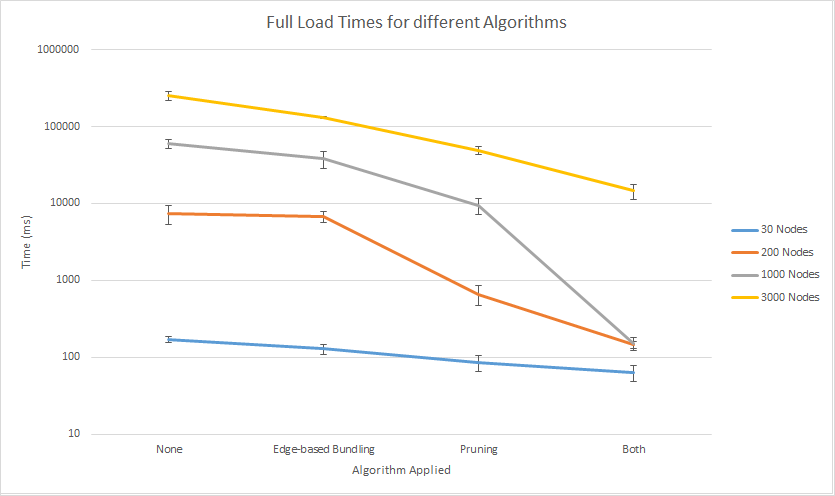
\includegraphics[width=15cm]{8/loadTimes}
    \caption{Load Times}
    \label{fig:loadTimes}
\end{figure}

Figure \ref{fig:packetSize} shows a steady decrease in packet size from no algorithm being applied, to Node Bundling based on number of edges, to Node Pruning, to applying Node Pruning then Node Bundling based on number of edges. It is again worth noting that the y-axis has a logarithmic scale.

\begin{figure}[H]
    \centering
    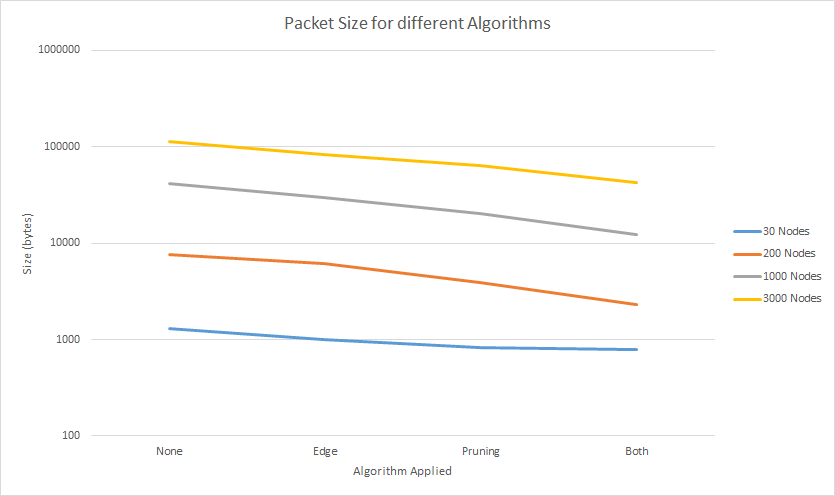
\includegraphics[width=15cm]{8/packetSize}
    \caption{Packet Size}
    \label{fig:packetSize}
\end{figure}

The above results clearly show the benefits of applying different algorithms to reduce the amount amount of data that is to be visualised in regards to both the amount of data that needs to be transferred and how long it takes to load a visualisation, from a user clicking `Load' to the network rendering. 

For 30 nodes, the amount of time saved when node bundling based on edges was 41ms, and for 3000 nodes the time saved was 120759ms (just over 2 minutes). The amount of time spent processing the networks on the server in order to get the stated time savings was 0.36ms for 30 nodes and 94ms for 3000 nodes. For node pruning, the time spent pruning on the server for 30 nodes was 0.38ms and resulted in an 84.8ms speed up, and for 3000 nodes the time spent pruning on the server was 169ms and the time saved in total was 203010ms (just over 3 and a third minutes). Finally, when applying both algorithms, there was 0.42ms spent processing the information on the server for 30 nodes, with a total time saving of 107ms, and 192ms applying the algorithms on 3000 nodes, with a time saving of 237177ms (just under 4 minutes). These results clearly show the benefit of applying the bundling algorithms.

It is worth noting that, despite the fact that performance increased greatly when applying the above algorithms, this is solely due to the fact that less nodes were shown. There are attempts to reduce the amount of data lost, both in attempting to remove the least critical nodes to the visualisation, and showing where nodes have been bundled and how many nodes have been bundled.

The full set of results can be seen in Appendix \ref{sec:perf-eval-tab}.

\end{document}